\documentclass[a4paper,12pt]{article}

\usepackage[utf8]{inputenc}
\usepackage[a4paper, left=3cm, right=3cm, top=3cm, bottom=3cm]{geometry}
\usepackage[frenchb]{babel}
\usepackage{default}
\usepackage{pslatex}
\usepackage{graphicx}
\usepackage{algorithmic}
\usepackage{multicol}
\usepackage{amsmath}
\usepackage{amssymb}
\usepackage{textcomp}
\usepackage{pgf}
\usepackage{tikz}
\usepackage{pgfplots}
\usepackage{capt-of}
\usepackage{esvect}
\usepackage[T1]{fontenc}

\title{Proposition pour le projet d'agenda collaboratif}
\author{Pleinet Estelle, Porteries Tristan}

\begin{document}

\maketitle

\tableofcontents

\section{Introduction}

Ce document est une proposition pour répondre au projet d'INFO 406.

\subsection{But}

Le point fort visé est le réseau crée autour du partage d'agendas.
Des utilisateurs pourraient donc créer et publier des agendas qui seront à leur suite suivis par des utilisateurs.

Les agendas suivis par les utilisateurs sont filtrés pour obtenir seulement les évenements interéssants puis regroupés en un seul agenda personnel.

Il s'agit d'une application pouvant être hors ligne avec des synchronisations des dernières modifications lorsque l'utilisateur retrouve une connexion.

\section{Entitées}

Il existe quatre types d'entitée dans ce système~: les utilisateurs, les groupes, les agendas et les évenements.

\subsection{Utilisateur}

Les utilisateurs sont uniques par la création de compte, ils peuvent gérer toutes les autres entitées selon le niveau de permission accordé.

Par exemple un membre d'association ayant accès à l'agenda de cette association pourra ajouter des évenements mais aussi faire de même sur son agenda personnel. Il modifiera tous les agendas avec les permissions nécessaires sans disctinction de contexte.

\subsection{Agenda}

Les agendas sont composés d'évenements ainsi que des liens vers des agendas à regrouper avec des filtres associés.
Chaque agenda contient une liste de ses modérateurs avec leur droit associés.

Pour l'exemple Paul veut suivre l'agenda d'une association mais ne peut pas venir aux réunions le mardi soir à cause de son travail, il va donc lier son agenda personnaliser avec celui de l'association mais avec le filtre spécifique excluant le mardi.

\subsection{Groupe}

Un groupe est une collection d'agenda d'une entitée réel e.g~: entreprise, association.
Ce groupe contient aussi une liste de membre ayant les droits d'ajouter ou supprimer un agenda du groupe ainsi que de modifier cette liste de membre.

Par exemple l'USMB serait un groupe proposant un agenda par section et professeur.

\section{Actions}

Cette section détaille les différentes actions possible entre les entitées. Il faut tout d'abord rappeler que l'application peut être utilisé hors ligne et a donc un ensemble d'actions plus restreins.

Toutes ces actions se regroupe sous 4 catégories~:

\begin{itemize}
	\item connexion / inscription~;
	\item gestion de compte~;
	\item gestion de groupe~;
	\item gestion d'agenda~;
\end{itemize}

\subsection{Connexion et inscription}

\begin{itemize}
	\item Un nouvel utilisateur doit pouvoir s'inscrire.
	\item Un utilisateur déjà inscrit doit pouvoir se connecter pour accèder à son agenda personnel ainsi que avoir la possibilité de modifier du contenu.
	\item Un utilisateur déjà inscrit doit aussi pouvoir se désinscrire.
\end{itemize}

\subsection{Gestion de compte}

\begin{itemize}
	\item Un utilisateur doit pouvoir voir son agenda personnel.
	\item Pouvoir lister les groupes liées à l'agenda personnel.
\end{itemize}

\subsection{Gestion de groupe}

\begin{itemize}
	\item Un utilisateur doit pouvoir créer un nouveau groupe.
	\item Pouvoir s'inscrire à un groupe.
	\item Avec les droits suffisant~:
	\begin{itemize}
		\item Ajouter un agenda dans le groupe~;
		\item Supprimer un agenda du groupe~;
		\item Modifier la liste des membres ainsi que leur droits.
	\end{itemize}
\end{itemize}

\subsection{Gestion d'agenda}

\begin{itemize}
	\item Ajouter et supprimer un evénement.
	\item Ajouter un lien vers un agenda distant avec un filtre.
	\item Lister les agendas distants liés et leur groupe / personne.
	\item Modifier le filtre d'un lien vers un agenda distant.
	\item Supprimer un lien vers un agenda distant.
\end{itemize}

\section{Diagramme}

\begin{center}
	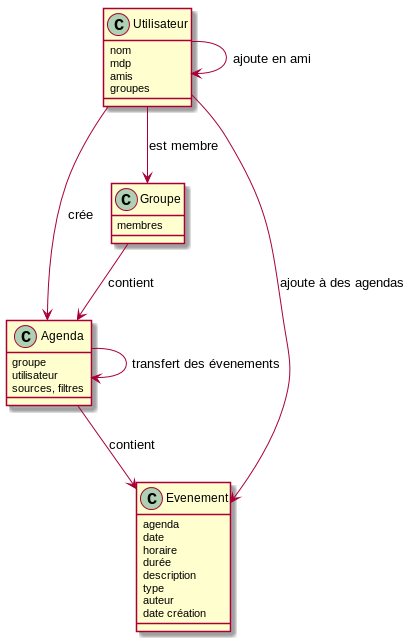
\includegraphics[width=13cm]{diagramme.png}
\end{center}

\section{Application}

Cette proposition se base sur une application pouvant fonctionner hors ligne donc non utilisée dans un navigateur. Par ces contraintes il est possible d'utiliser le language de notre choix tant qu'il possèdent des librairies pour les communications par réseau et les interfaces graphiques.
Le java et le python sont deux candidats et tous les deux sont pratiqués par les membres du groupe.

\subsection{Protocole d'échange}

Le protocole XML-RPC semble le plus adapter pour l'échange d'information dans le cadre de ce type d'application. Ce protocole ne transfert que les données sous forme XML avec une conservation assez large du typage ce qui pourrait permettre d'éviter la conversion du côté serveur et client à chaque bout de la communication.

Les échanges se feront grâce à des numéros de session obtenu lors d'une connexion puis passé en argument de toutes les autres fonctions après pour obtenir certain droits particuliers.

\begin{itemize}
	\item $connection(login, mdp) -> session\_id$
	\item $acces\_ou\_modification\_donnee(session\_id, *)$
\end{itemize}


\subsection{Language}

XML-RPC est disponible en python dans la module xmlrpclib (natif ?).

\section{Questions}

\begin{itemize}
	\item Faudrait il avoir plusieurs agendas personels par utilisateur ?
	\item Comment partager un agenda personnel ?
\end{itemize}


\end{document}
